\documentclass{article} % For LaTeX2e
\usepackage[final]{colm2025_conference}
\usepackage{graphicx}
\usepackage{amsmath}
\usepackage{microtype}
\usepackage{hyperref}
\usepackage{url}
\usepackage{booktabs}
\usepackage{lineno}
\usepackage{amsmath}
\usepackage{algpseudocode}
\usepackage{algorithm}

\definecolor{darkblue}{rgb}{0, 0, 0.5}
\hypersetup{colorlinks=true, citecolor=darkblue, linkcolor=darkblue, urlcolor=darkblue}

\usepackage{etoolbox}
\makeatletter
\patchcmd{\@maketitle}
  {Published as a conference paper at COLM 2025}
  {}
  {}
  {}
\makeatother
\title{Week 3 Report}

% Authors must not appear in the submitted version. They should be hidden
% as long as the \colmfinalcopy macro remains commented out below.
% Non-anonymous submissions will be rejected without review.

\author{Mu Junrong}

% The \author macro works with any number of authors. There are two commands
% used to separate the names and addresses of multiple authors: \And and \AND.
%
% Using \And between authors leaves it to \LaTeX{} to determine where to break
% the lines. Using \AND forces a linebreak at that point. So, if \LaTeX{}
% puts 3 of 4 authors names on the first line, and the last on the second
% line, try using \AND instead of \And before the third author name.

\newcommand{\fix}{\marginpar{FIX}}
\newcommand{\new}{\marginpar{NEW}}

\begin{document}

\ifcolmsubmission
\linenumbers
\fi

\maketitle

\begin{abstract}
This report focuses on the mathematics involved, 
the background about the environment (CartPole), as well as the results obtained.
\end{abstract}

\section{Mathmetics involved}
From Week 2's Report section 4, in Reinforcement Learning, the agent learns a policy \(\pi : \mathcal{S} \to \mathcal{A}\) 
that maximizes expected return (\cite{sutton2018reinforcement}):
\[G_t = \sum_{k=0}^\infty \gamma^k R_{t+k+1}\]
The main objective of Reinforcement Learning (RL) is to find an optimal policy $\pi$ that maximizes the reward (i.e. maximizes the state-value function and action-value function) (\cite{sutton1999policy}):
\[
\pi^{*} = \arg \max_{\pi} \mathbb{E}_{\pi} \left[ \sum_{t=0}^{\infty} \gamma^t R_{t+1} | \pi \right]
\]

\subsection{Objective function}
From section 5.1 and 5.2, the objective function of Reinforcement Learning is defined as
\[
J(\theta) = \mathbb{E}_{\tau \sim \pi_{\theta}} \left[ \sum_{t=0}^{T} \gamma^{t} r_{t} \right]
\]
where \(\tau\) represent a trajectory (i.e., the sequence of states, actions, rewards):

\[
\tau = (s_0, a_0, r_1, s_1, a_1, r_2, \ldots)
\]
By differentiating the objective function \(J(\theta)\):
\begin{align*}
\nabla_\theta J(\theta) &= \nabla_\theta \int p_\theta(\tau) R(\tau) \,d\tau \\
&= \int \nabla_\theta p_\theta(\tau) R(\tau) \,d\tau \\
&= \mathbb{E}_{\tau \sim \pi_\theta} \left[ \nabla_\theta \log p_\theta(\tau) R(\tau) \right]
\end{align*}

\subsection{Basic policy gradient}
From section 5.3, the trajectory probability under the policy is given by
\[p_\theta(\tau) = p(s_0) \prod_{t=0}^{T} \pi_\theta(a_t|s_t) p(s_{t+1}|s_t, a_t)\]

\[\log p_\theta(\tau) = \sum_{t=0}^{T} \log \pi_\theta(a_t|s_t) + \text{C}\]

By substituting into the objective function, the basic policy gradient formula is derived
\[
\nabla_\theta J(\theta) = \mathbb{E}_{\tau \sim \pi_\theta} \left[ \left( \sum_{t=0}^T \nabla_\theta \log \pi_\theta (a_t | s_t) \right) R(\tau) \right]
\]

Therefore, in the algorithm, the policy parameters are updated using gradient ascent
    \[
    \theta \leftarrow \theta + \alpha \cdot \nabla_{\theta} J(\theta)
    \]
where $\alpha$ is the learning rate.

\section{Background of the environment}
CartPole is a physics-based control problem. It simulates a cart on a track which can move left and right. There is a pole (e.g. inverted pendulum) that starts upright on the cart, but can fall to either side. The goal of the agent is to keep the pole balanced upright by moving the cart left or right.

\subsection{Key definitions in CartPole}
The state space $\mathcal{S}$ is a finite set of 4-dimensional vectors:
\[
\mathcal{S} \subseteq \mathbb{R}^4 \quad \text{where} \quad \mathbf{s}_t = \begin{pmatrix}
x_t & \dot{x}_t & \theta_t & \dot{\theta}_t
\end{pmatrix}^\top
\]
with components:
\begin{itemize}
    \item $x_t$: Cart position
    \item $\dot{x}_t$: Cart velocity
    \item $\theta_t$: Pole angle (in radians)
    \item $\dot{\theta}_t$: Pole angular velocity
\end{itemize}

The action space $\mathcal{A}$ is a discrete set:
\[
\mathcal{A} = \{0, 1\} \quad \text{where} \quad 
\begin{cases}
0 = \text{``move left''} \\
1 = \text{``move right''}
\end{cases}
\]

The reward function $R: \mathcal{S} \times \mathcal{A} \to \mathbb{R}$ provides:
\[
r(\mathbf{s}_t, a_t) = +1 \quad \text{for every timestep the pole remains balanced}
\]

A trajectory $\tau = (\mathbf{s}_0, a_0, \mathbf{s}_1, a_1, \dots)$ terminates when either:
\begin{itemize}
    \item The pole falls: $|\theta_t| > \theta_\text{max}$ ($\approx 12^\circ$ or 0.209 rad)
    \item The cart moves out of bounds: $|x_t| > x_\text{max}$ (typically 2.4 m)
\end{itemize}

\subsection{Aim of the agent}
The agent must learn a policy (a way to choose left or right) that keeps the pole upright as long as possible. Since it gets a reward of +1 per timestep, the agent is incentivized to stay balanced longer.

\section{Result of the experiment}
This experiment evaluates the performance of Vanilla policy gradient (VPG) methods in the CartPole-v0 environment, focusing on two key design choices: Reward-to-go (RTG) vs. non-RTG return estimation and small batch (1,000 steps) vs. large batch (4,000 steps) training. The goal is to analyze how RTG and batch size affect sample efficiency (i.e., learning speed), final performance (i.e., maximum achievable return) and training stability (i.e., variance in returns).

In conclusion, large batch data with reward-to-go (RTG) yield the best performance (i.e., highest return, low variance and less fluctuation). In general, large batch data and reward-to-go (RTG) yield better results than smaller batch data and without reward-to-go.


\subsection{Variance in return}
Based on Figure 1 and Figure 2, the learning curves of data with reward-to-go are smoother, with fewer oscillations and swings, indicating lower variance. Thus, the reward-to-go method reduces the variance, ensuring stability.
\begin{figure}[H]
    \centering
    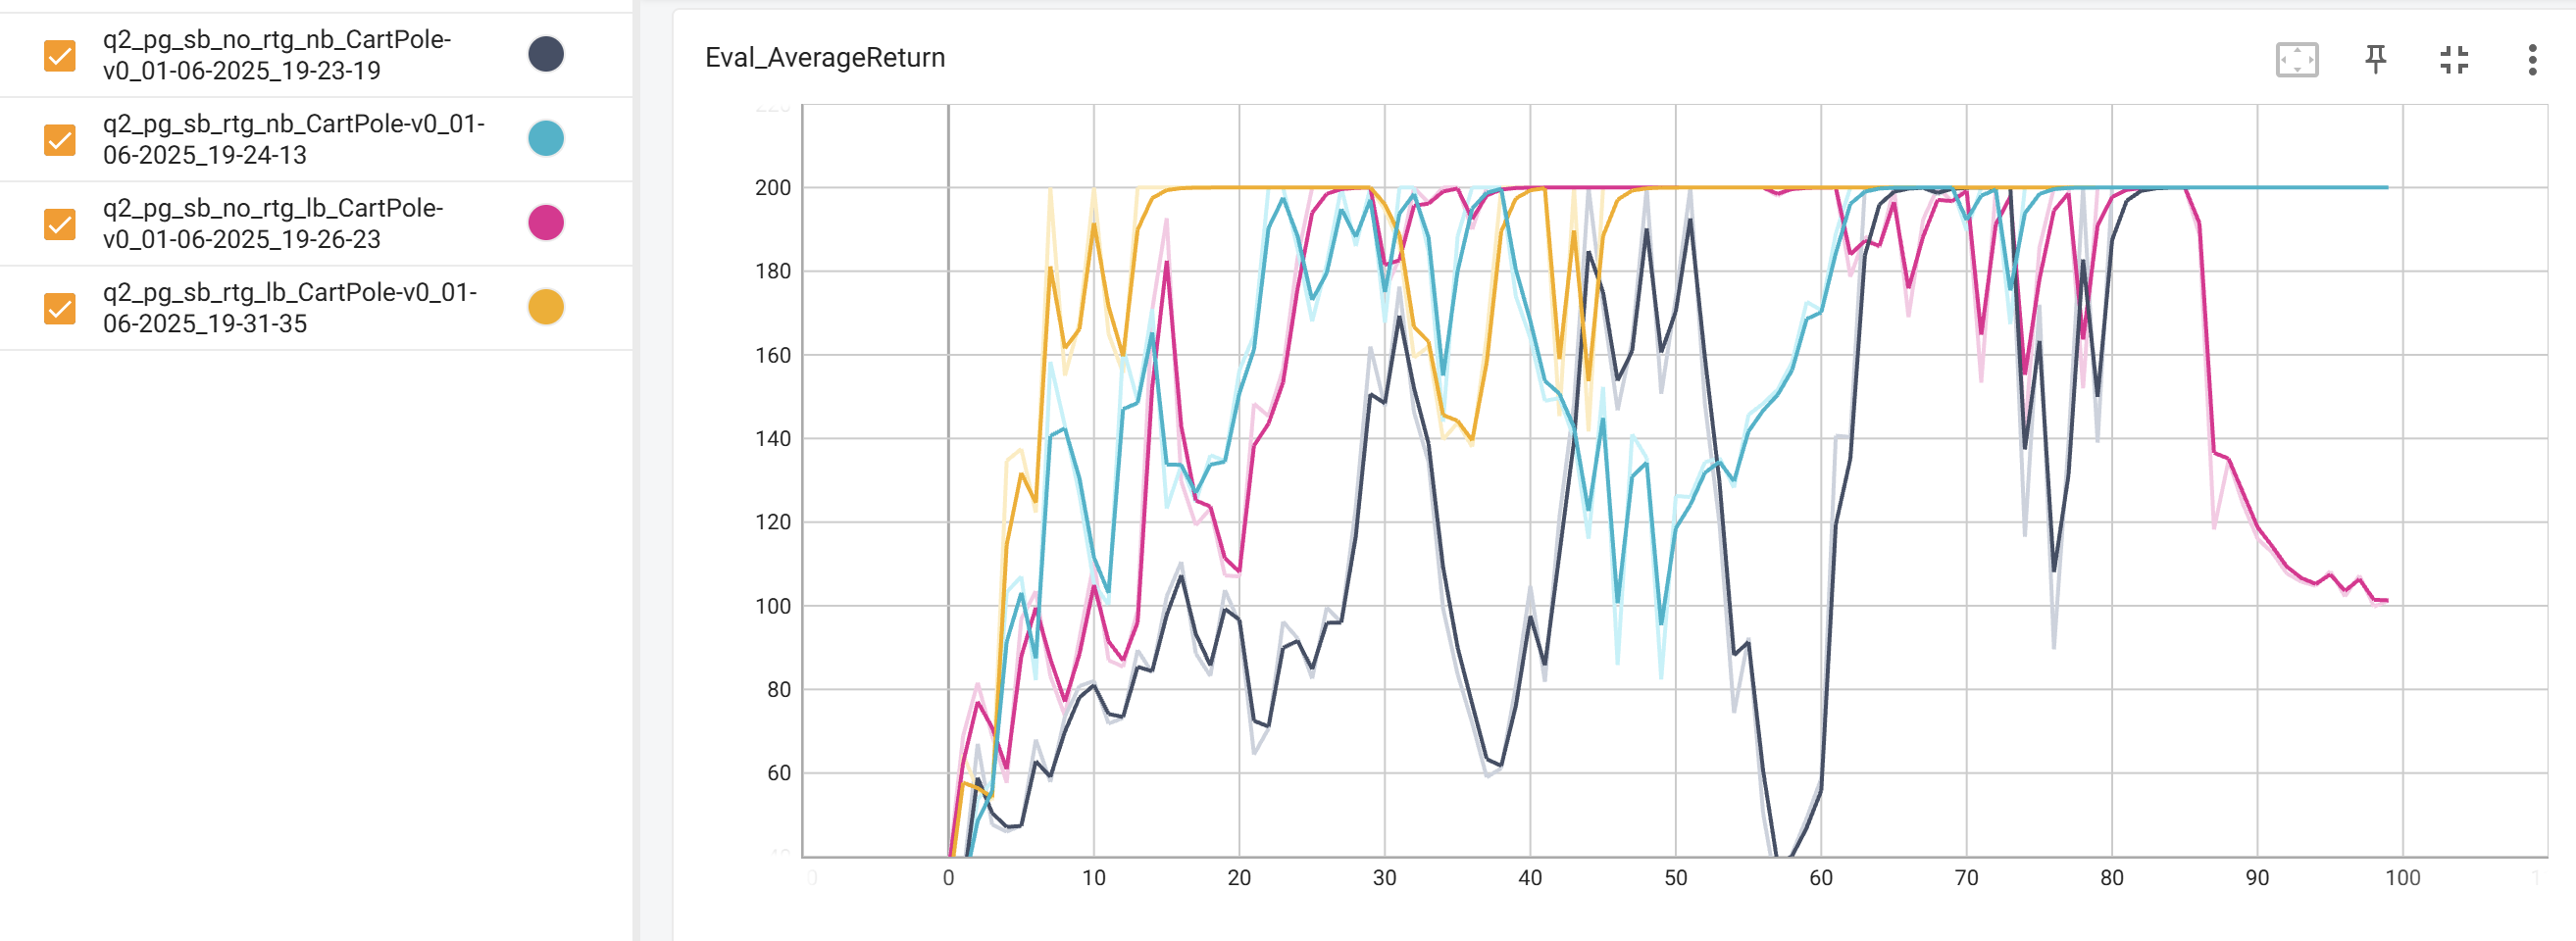
\includegraphics[width=1\linewidth]{eval_AverageReturn.png}
    \caption{Learning curve of average return over training steps.}
    \label{fig:average}
\end{figure}
\begin{figure}[H]
    \centering
    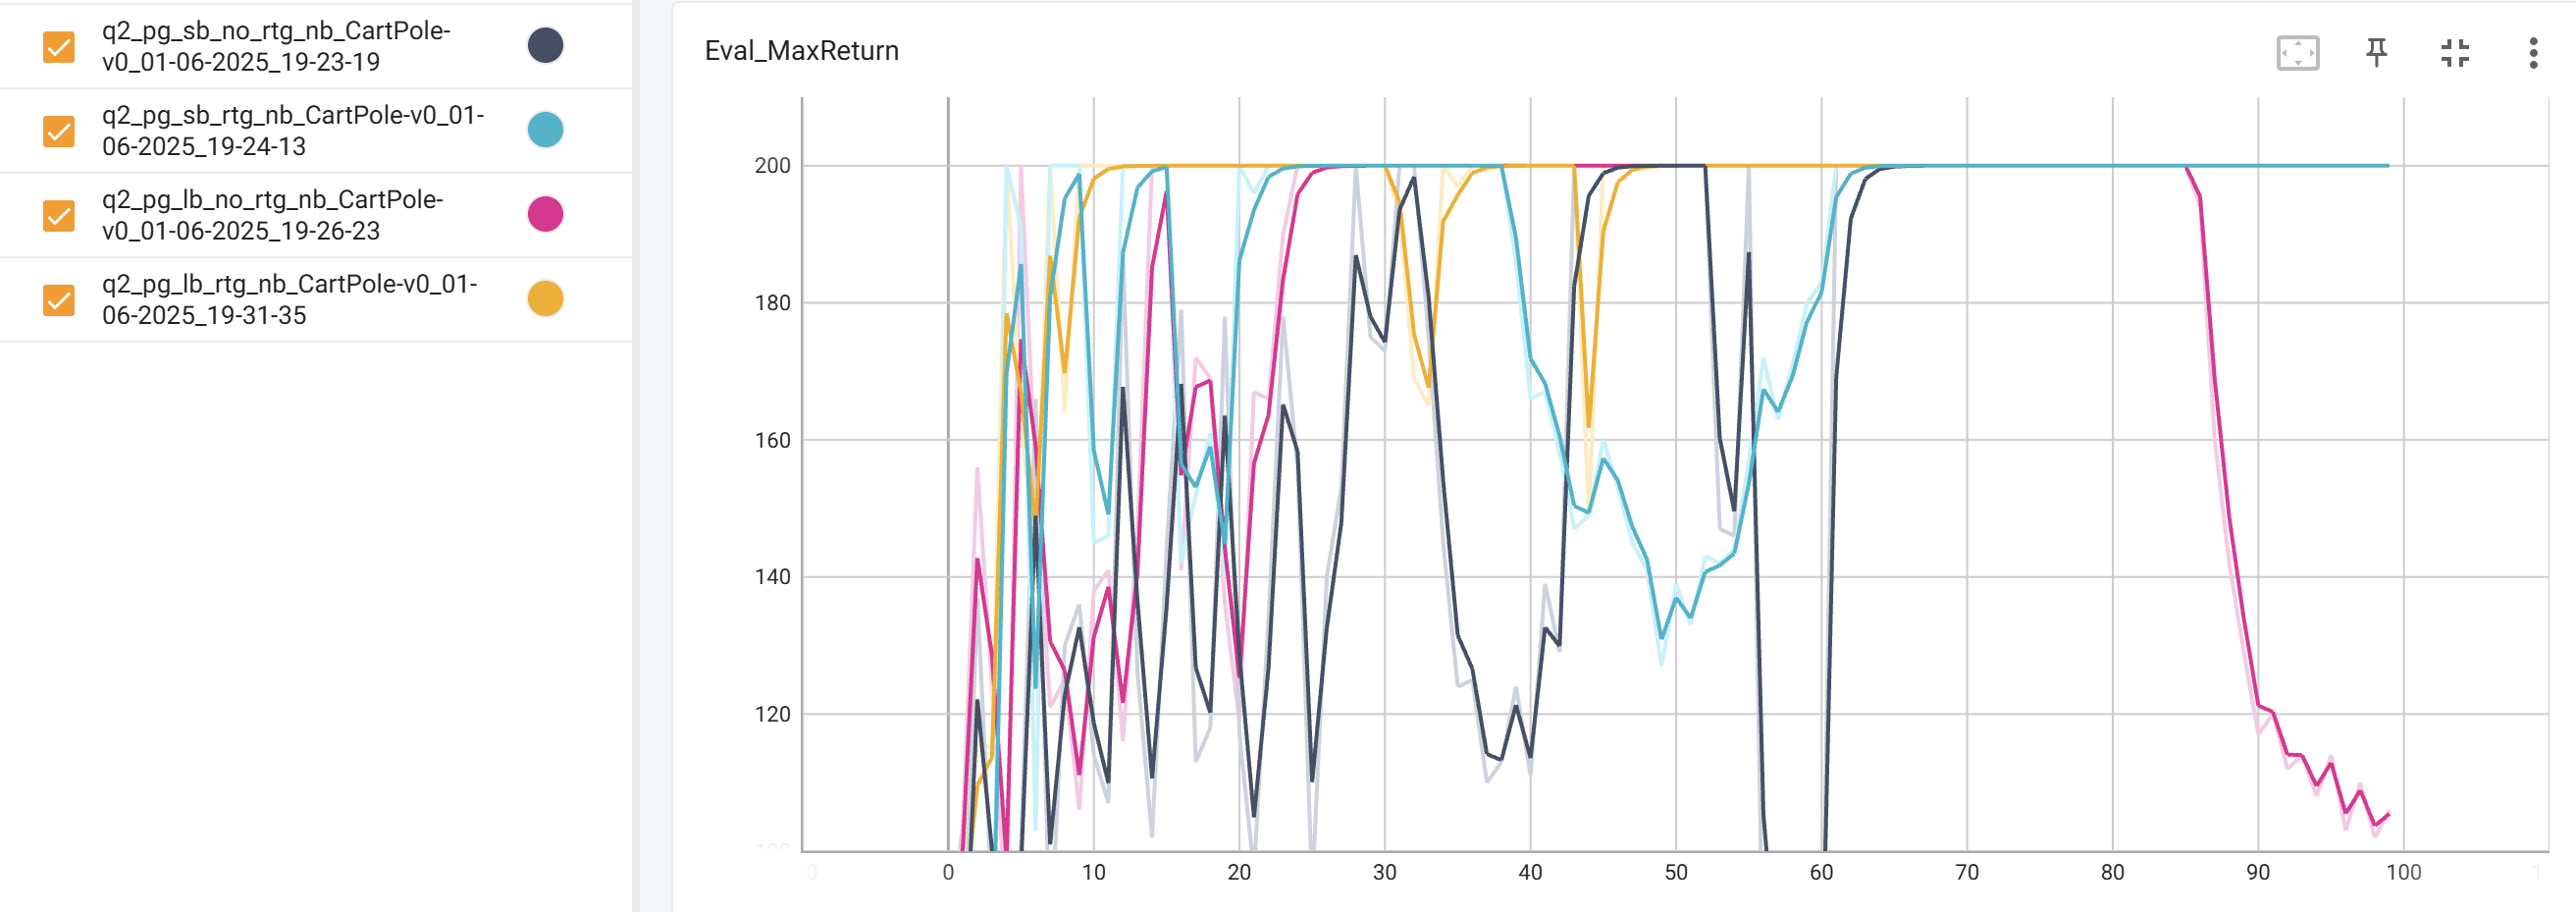
\includegraphics[width=1\linewidth]{Eval_MaxReturn.png}
    \caption{Learning curve of maximum return over training steps.}
    \label{fig:max}
\end{figure}
\subsection{Learning speed and final performance}
Based on Figure 1 and Figure 2, all four experiments reach 200 (the maximum achievable for CartPole-v0) as the training steps increase. Based on Figure 3, the actor loss is decreasing steadily since the policy is learning to increase the expected return. Especially for large batch data without reward-to-go, the curve experiences a sharp decrease around the time step = 80, possibly because of a quick learning where the reward is.
However, large batch data with reward-to-go converges to 200 faster, and the loss decreases at a faster rate.  
\begin{figure}[H]
    \centering
    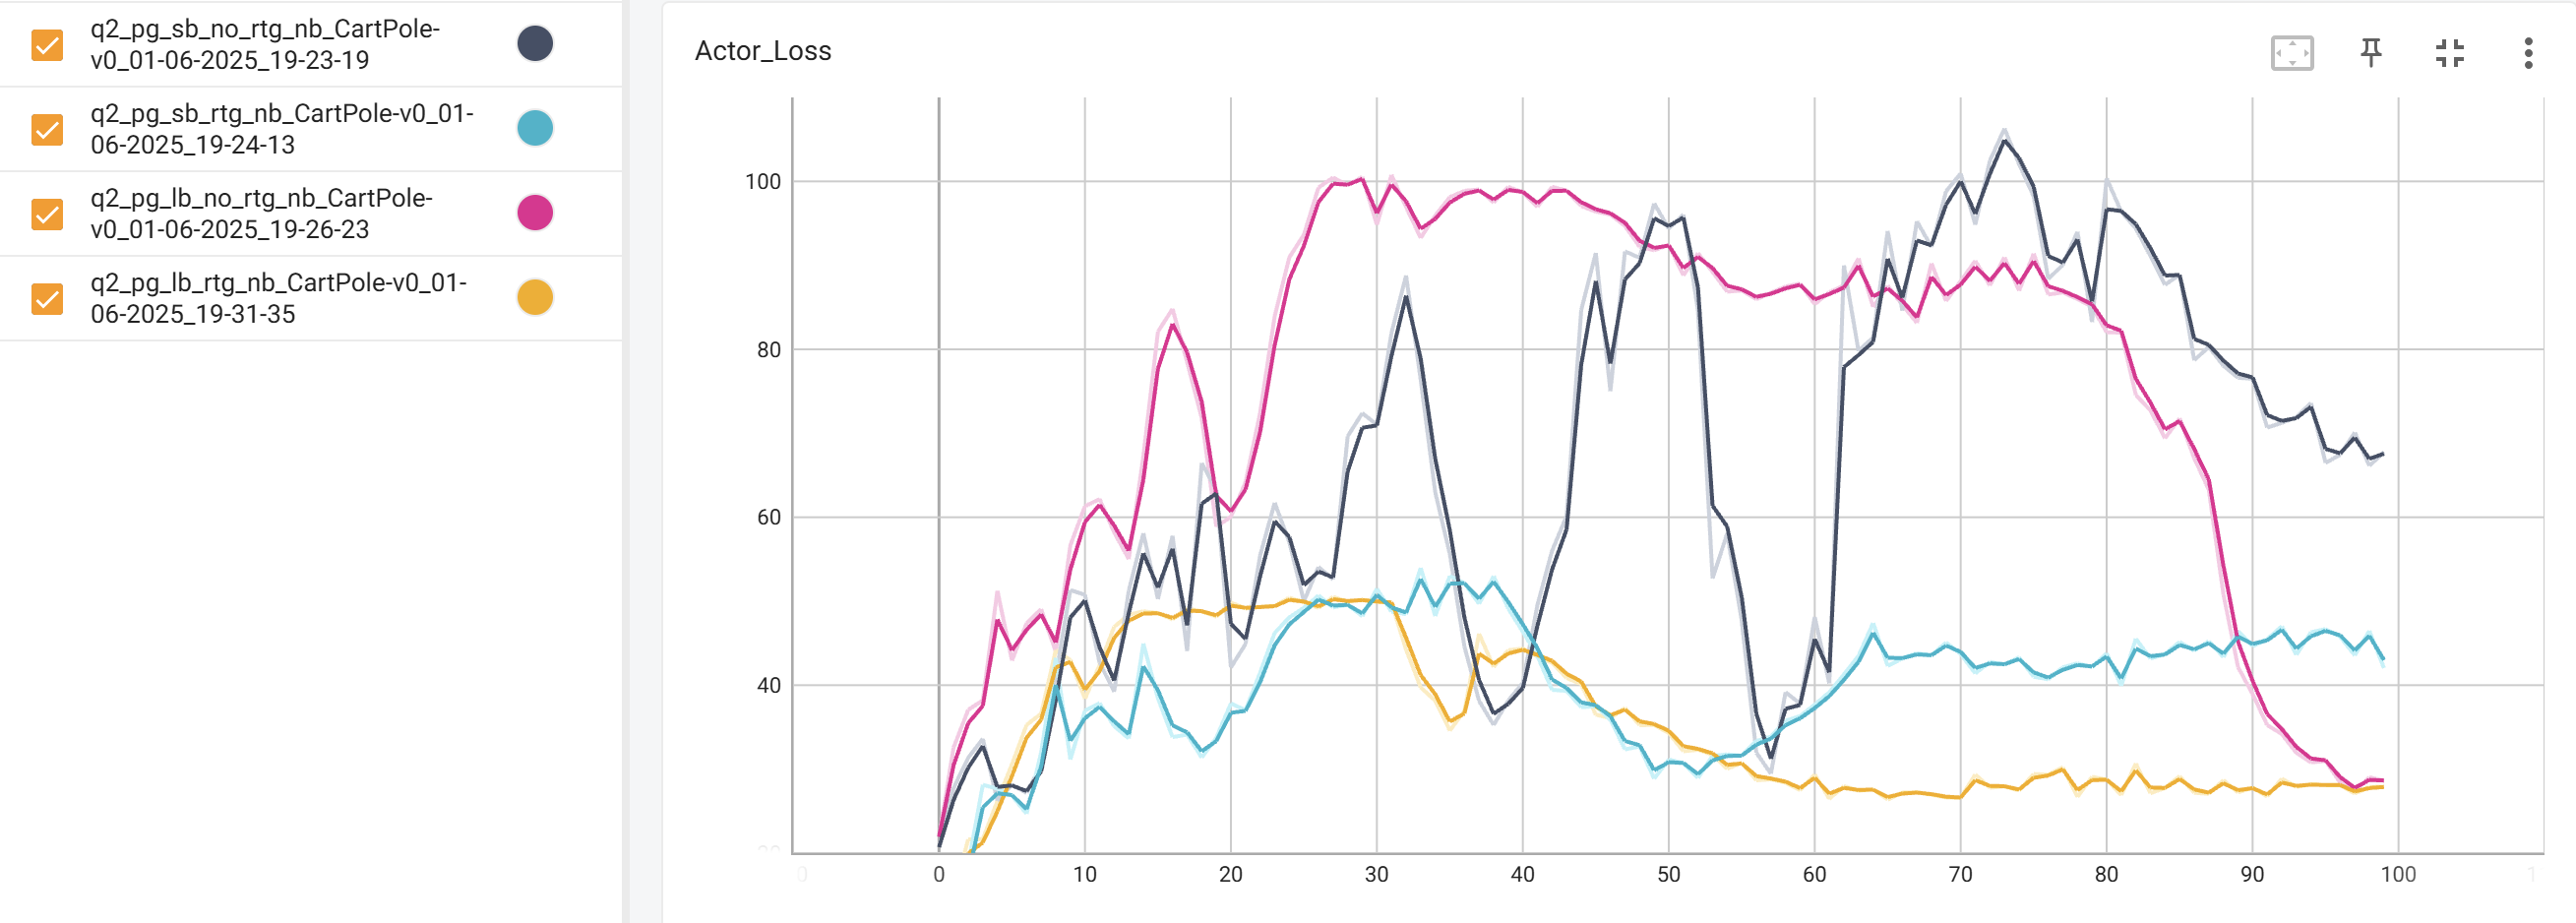
\includegraphics[width=1\linewidth]{Actor_Loss.png}
    \caption{Learning curve of actor loss over training steps.}
    \label{fig:loss}
\end{figure}


\bibliography{colm2025_conference}
\bibliographystyle{colm2025_conference}


\end{document}
